% TU Delft beamer template
% Author: Erwin Walraven (initial version was created by Maarten Abbink)
% Delft Universiy of Technology

\documentclass{beamer}
\usepackage[english]{babel}
\usepackage{calc}
\usepackage[absolute,overlay]{textpos}
\usepackage{graphicx}
\graphicspath{ {./images/} }
\usepackage{subfig}
\usepackage{amsmath}
\usepackage{amsfonts}
\usepackage{amsthm}
\usepackage{mathtools}
\usepackage{comment}
\usepackage{float}
\usepackage{epstopdf}
\usepackage{braket}
\usepackage{MnSymbol,wasysym}
\usepackage{physics}

\setbeamertemplate{navigation symbols}{} % remove navigation symbols
\mode<presentation>{\usetheme{tud}}

% BIB SETTINGS
\usepackage[backend=bibtex,firstinits=true,maxnames=30,maxcitenames=20,url=false,style=authoryear]{biblatex}
\bibliography{bibfile}
\setlength\bibitemsep{0.3cm} % space between entries in the reference list
\renewcommand{\bibfont}{\normalfont\scriptsize}
\setbeamerfont{footnote}{size=\tiny}
\renewcommand{\cite}[1]{\footnote<.->[frame]{\fullcite{#1}}}

\newcommand{\V}{\mathbb{V}}
\newcommand{\valk}{\text{k}}
\newcommand{\veck}{\textbf{k}}

\title[]{The Fermi Hole}
\institute[]{Delft University of Technology, The Netherlands}
\author{Ivan Kulesh \and Martijn Papendrecht}
%\date{}

\begin{document}
{
\setbeamertemplate{footline}{\usebeamertemplate*{minimal footline}}
\frame{\titlepage}
}

{\setbeamertemplate{footline}{\usebeamertemplate*{minimal footline}}

}

\begin{frame}{Some properties of Fermi gas}
  Particles dwell in a large but finite volume $\mathcal{V}$.
\end{frame}


%!TeX spellcheck = en-US,en-DE

\begin{frame}[t]{Calculating sum}
  \vspace{0.5cm}
  To continue we need to find
  \only<1,3,4,5>{
    \begin{equation*}
      \begin{gathered}
        F(\valk, \vecr) = \frac{1}{\mathcal{V}} \sum_{\veck} e^{- i \textbf{k}\vecr}
        \bra{g} \hat c^{\dagger}_{\textbf{k}\sigma} \hat c_{\textbf{k}\sigma} \ket{g}
      \end{gathered}
    \end{equation*}
  }
  \only<2>{
    \begin{equation*}
      \begin{gathered}
        F(\valk, \vecr) = \frac{1}{\mathcal{V}} \sum_{\veck} e^{- i \textbf{k}\vecr}\:
        \textcolor{red}{
        \bra{g} \hat c^{\dagger}_{\textbf{k}\sigma} \hat c_{\textbf{k}\sigma} \ket{g}
        }
      \end{gathered}
    \end{equation*}
  }
  \only<3>{
    \begin{block}{Number of particles operator}
      $$ \hat c^{\dagger}_{\textbf{k}\sigma} \hat c_{\textbf{k}\sigma} = \hat n_{\textbf{k}\sigma}$$
    \end{block}
    %\vspace{0.5cm}
    \begin{equation*}
      \bra{g} \hat c^{\dagger}_{\textbf{k}\sigma} \hat c_{\textbf{k}\sigma} \ket{g} =
      \bra{g} \hat n_{\textbf{k}\sigma} \ket{g} =
      \begin{cases}
        1 \quad \valk \leq \valk_F\\
        0 \quad \valk > \valk_F
      \end{cases}
    \end{equation*}
  }

  \only<4>{
    \vspace{0.5cm}
    Heaviside step function
    \begin{equation*}
      \bra{g} \hat c^{\dagger}_{\textbf{k}\sigma} \hat c_{\textbf{k}\sigma} \ket{g} =
      H(\valk_F - \abs{\veck})
    \end{equation*}
  }

  \only<5>{
    \vspace{0.5cm}
    Change to summation inside the Fermi sphere
    \begin{equation*}
      F(\valk, \vecr) = \frac{1}{\mathcal{V}} \sum_{\abs{\veck}\leq \valk_F} e^{- i \textbf{k}\vecr}
    \end{equation*}
  }

\end{frame}

\begin{frame}{From summation to integration}
  Multiply and divide by unit cell volume
  \begin{equation*}
    F(\valk, \vecr) = \frac{1}{\mathcal{V}} \sum_{\abs{\veck}\leq \valk_F} e^{- i \textbf{k}\vecr} =
    \frac{1}{\mathcal{V}} \frac{\mathcal{V}}{ 8 \pi^3} \sum_{\abs{\veck}\leq \valk_F} e^{- i \textbf{k}\vecr} d^3\valk
  \end{equation*}
  \vspace{0.5cm}
  In the limit $\mathcal{V} \to \infty$
  \begin{equation*}
    F(\valk, \vecr) = \frac{1}{8 \pi^3} \sum_{\abs{\veck}\leq \valk_F} e^{- i \textbf{k}\vecr} d^3\valk
    \to
    \frac{1}{8 \pi^3} \int_{\abs{\veck}\leq \valk_F} e^{- i \textbf{k}\vecr} d^3\valk
  \end{equation*}
\end{frame}

\begin{frame}[t]{Evaluation of the integral}
  \vspace{0.2cm}
  We will integrate in spherical coordinates
  \only<1>{
    \begin{equation*}
      F(\valk, \vecr) = \frac{1}{8 \pi^3} \int_{\abs{\veck}\leq \valk_F} e^{- i \textbf{k}\vecr} d^3\valk
    \end{equation*}
  }
  \only<2>{
  \begin{equation*}
    F(\valk, \vecr) =
    \frac{1}{8 \pi^3} \int_{\valk = 0}^{\valk_F} \int_{\theta = 0}^{\pi} \int_{\phi = 0}^{2 \pi}
    e^{- i \text{k}r\cos{\theta}}\text{k}^2\sin{\theta} \: d \phi d\theta d \text{k}
  \end{equation*}
  }
  \vfill
  \begin{figure}
    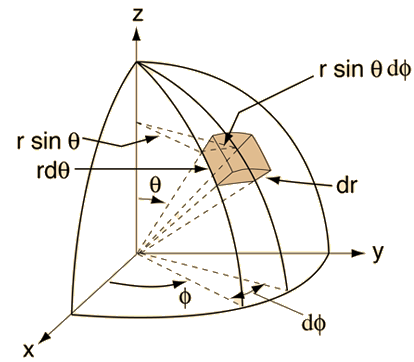
\includegraphics[height=4cm]{sphcoordel}
    %\caption{}
    \label{sphcoordel}
  \end{figure}
\end{frame}

\begin{frame}{Evaluation of the integral}
  Integration over $\phi$

  % \only<>{
  % \begin{equation*}
  %   F(\valk, \vecr) =
  %   \frac{1}{8 \pi^3} \int_{\valk = 0}^{\valk_F} \int_{\theta = 0}^{\pi} \int_{\phi = 0}^{2 \pi}
  %   e^{- i \text{k}r\cos{\theta}}\text{k}^2\sin{\theta} \: d \phi d\theta d \text{k}
  % \end{equation*}
  % }

  \only<1>{
  \begin{equation*}
    F(\valk, \vecr) =
    \frac{1}{8 \pi^3} \int_{\valk = 0}^{\valk_F} \int_{\theta = 0}^{\pi}
    \textcolor{red}{\int_{\phi = 0}^{2 \pi}}
    e^{- i \text{k}r\cos{\theta}}\text{k}^2\sin{\theta} \: \textcolor{red}{d \phi} d\theta d \text{k}
  \end{equation*}
  }

  \only<1>{
  \begin{equation*}
    F(\valk, \vecr) =
    \frac{1}{4 \pi^2} \int_{\valk = 0}^{\valk_F} \int_{\theta = 0}^{\pi}
    e^{- i \text{k}r\cos{\theta}}\text{k}^2\sin{\theta} \: d\theta d \text{k}
  \end{equation*}
  }

\end{frame}

\begin{frame}{Evaluation of the integral}
  Integration over $\theta$

  \only<1,2>{
  \begin{equation*}
    F(\valk, \vecr) =
    \frac{1}{4 \pi^2} \int_{\valk = 0}^{\valk_F} \textcolor{red}{\int_{\theta = 0}^{\pi}}
    e^{- i \text{k}r\textcolor{red}{\cos{\theta}}}\text{k}^2
    \textcolor{red}{\sin{\theta} \: d\theta} d \text{k}
  \end{equation*}
  }

  \only<1,2>{
  \begin{equation*}
    F(\valk, \vecr) =
    \frac{1}{4 \pi^2} \int_{\valk = 0}^{\valk_F} \textcolor{red}{\int_{\theta = 0}^{\pi}}
    e^{- i \text{k}r\textcolor{red}{\cos{\theta}}}\text{k}^2 \: \textcolor{red}{-d\cos{\theta}} d \text{k}
  \end{equation*}
  }

  \only<1>{
  \begin{equation*}
    F(\valk, \vecr) =
    \frac{1}{4 \pi^2} \int_{\valk = 0}^{\valk_F} \textcolor{red}{\int_{\eta = -1}^{1}}
    e^{i \text{k}r\textcolor{red}{\eta}}\text{k}^2 \: \textcolor{red}{d\eta} d \text{k}
  \end{equation*}
  }

  \only<2>{
  \begin{equation*}
    F(\valk, \vecr) =
    \frac{1}{4 \pi^2} \int_{\valk = 0}^{\valk_F}
    \frac{2}{\text{k}r}\sin{(\text{k}r)} \: \text{k}^2 \: d \text{k}
  \end{equation*}
  }

\end{frame}

\begin{frame}[t]{Evaluation of the integral}
  \vspace{0.3cm}
  Integration over k

  \begin{equation*}
    F(\valk, \vecr) =
    \frac{1}{4 \pi^2} \int_{\valk = 0}^{\valk_F}
    \frac{2}{\text{k}r}\sin{(\text{k}r)} \: \text{k}^2 \: d \text{k} =
    \frac{1}{2 \pi^2 r^3} \int_{\valk = 0}^{\valk_F}
    \sin{(\text{k}r)} \: \text{k} r \: d \text{k}r
  \end{equation*}

  \only<1>{
  \begin{equation*}
    F(\valk, \vecr) =
    \frac{1}{2 \pi^2 r^3} \left \{ \sin(\valk_F r) - \valk_F r \cos(\valk_F r) \right \}
  \end{equation*}
  }

  \only<2>{
  \begin{equation*}
    F(\valk, \vecr) =
    \frac{\valk_F^3}{2 \pi^2 r^3 \valk_F^3} \left \{ \sin(\valk_F r) - \valk_F r \cos(\valk_F r) \right \}
  \end{equation*}

  \begin{block}{Fermi wavenumber}
    $$ \valk_F^3 = \frac{3 \pi^2 N}{\V}$$
  \end{block}
  }
\end{frame}

\begin{frame}{Evaluation of the integral}
  \begin{equation*}
    \frac{1}{\mathcal{V}} \sum_{\veck} e^{- i \textbf{k}\vecr}
    \bra{g} \hat c^{\dagger}_{\textbf{k}\sigma} \hat c_{\textbf{k}\sigma} \ket{g} =
    \left ( \frac{N}{2\mathcal{V}} \right )
    \frac{3 \left \{ \sin(\valk_F r) - \valk_F r \cos(\valk_F r) \right \} }{(k_F r)^3}
  \end{equation*}

  \vspace{1cm}
  No divergence at zero: at $\valk_F r \to 0 \iff r \ll \lambda_F$
  \begin{equation*}
    3 \frac{\sin(k_F r) - k_F r \cos(k_F r)}{(k_F r)^3} \approx
    3 \frac{x - x^3/6 - x (1 - x^2/2)}{x^3} = \frac{3}{3} = 1
  \end{equation*}
\end{frame}


\begin{frame}{Title}
Begin with the equations.
\end{frame}

\begin{frame}
\def\x{\textbf{x}}
\def\V{\mathcal{V}}
\begin{align*}
\ket{\phi_\sigma(\x)} &= \hat{\psi}_\sigma(\x)\ket{g} \\
\hat{\psi}_\sigma(\x) &= \sum_k \hat{c}_{k,\sigma} \psi_{k,\sigma}(\x) \\
\psi_{k}(\vec{x}) &= \frac{1}{\sqrt{\V}} e^{-i\vec{k} \cdot \vec{x}}
\end{align*}

\begin{align*}
\bra{\phi_\sigma(\x)}\hat{\psi}_{\sigma'}^\dagger(\x')\hat{\psi}_{\sigma'}(\x')\ket{\psi_\sigma(\x)} \\
\bra{g}\hat{\psi}_\sigma^\dagger(\x)\hat{\psi}_{\sigma'}^\dagger(\x')\hat{\psi}_{\sigma'}(\x')\hat{\psi}_\sigma(\x)\ket{g} \\
\bra{g}\sum_k c_{k,\sigma}^\dagger \psi_{k,\sigma}^\ast(\x) \sum_{l} c_{l,\sigma'}^\dagger \psi_{l,\sigma'}^\ast (\x') \sum_m c_{m,\sigma'} \psi_{m,\sigma'}(\x') \sum_n c_{n,\sigma} \psi_{n,\sigma}(\x) \ket{g}
\end{align*}

Now we see two creation and two annihilation operators, but N should be conserved, so there are two cases:
\begin{equation}
\begin{split}
k,\sigma = m,\sigma' \\
l,\sigma' = n,\sigma
\end{split}
\end{equation}
\begin{equation}
\begin{split}
k,\sigma = n,\sigma \\
l,\sigma' = m,\sigma'
\end{split}
\end{equation}

In case $1$ we see $\sigma = \sigma'$ and $k=m, l=n$ so we reduce to:
\begin{align*}
\bra{g}\sum_k c_{k}^\dagger \psi_{k}^\ast(\x) \sum_{l} c_{l}^\dagger \psi_{l,}^\ast (\x') \sum_k c_{k} \psi_{k}(\x') \sum_l c_{l} \psi_{l}(\x) \ket{g} \\
-\bra{g}\sum_k c_{k}^\dagger \psi_{k}^\ast(\x)  \sum_k c_{k} \psi_{k}(\x') \sum_{l} c_{l}^\dagger \psi_{l}^\ast (\x') \sum_l c_{l} \psi_{l}(\x) \ket{g} \\
-\bra{g}\sum_k c_{k}^\dagger \psi_{k}^\ast(\x) c_{k} \psi_{k}(\x') \sum_{l} c_{l}^\dagger \psi_{l}^\ast (\x') c_{l} \psi_{l}(\x) \ket{g} \\
-\bra{g}\sum_k c_{k}^\dagger c_{k} \psi_{k}^\ast(\x) \psi_{k}(\x') \sum_{l} c_{l}^\dagger  c_{l}\psi_{l}^\ast (\x') \psi_{l}(\x) \ket{g} \\
-\bra{g}\sum_k c_{k}^\dagger c_{k} \frac{1}{\sqrt{\V}} e^{i\vec{k}\cdot\x} \frac{1}{\sqrt{\V}}e^{-i\vec{k}\cdot\x'} \sum_{l} c_{l}^\dagger  c_{l} \frac{1}{\sqrt{\V}}e^{i\vec{l}\cdot\x'} \frac{1}{\sqrt{\V}}e^{-i\vec{l}\cdot\x}\ket{g} \\
\frac{-1}{\V^2}\bra{g}\sum_k c_{k}^\dagger c_{k} e^{i\vec{k}\cdot(\x-\x')} \sum_{l} c_{l}^\dagger  c_{l} e^{i\vec{l}\cdot(\x'-\x)} \ket{g} \\
-\frac{1}{\V}\sum_k e^{i\vec{k}\cdot(\x-\x')} \bra{g} c_{k}^\dagger c_{k} \ket{g} \frac{1}{\V} \sum_l e^{i\vec{l}\cdot(\x'-\x)} \bra{g} c_{l}^\dagger  c_{l} \ket{g} \\
-9\left(\frac{N}{2\V}\right)^2 \left( \frac{\sin(k_Fr) - k_Fr \cos(k_Fr)}{(k_Fr)^3}\right)^2
\end{align*}

In case $2$ we see $k=n, l=m$ so we reduce to:
\begin{align*}
\bra{g}\sum_k c_{k,\sigma}^\dagger \psi_{k,\sigma}^\ast(\x) \sum_{l} c_{l,\sigma'}^\dagger \psi_{l,\sigma'}^\ast (\x') \sum_l c_{l,\sigma'} \psi_{l,\sigma'}(\x') \sum_k c_{k,\sigma} \psi_{k,\sigma}(\x) \ket{g} \\
+\bra{g}\sum_k c_{k,\sigma}^\dagger \psi_{k,\sigma}^\ast(\x) \sum_k c_{k,\sigma} \psi_{k,\sigma}(\x) \sum_{l} c_{l,\sigma'}^\dagger \psi_{l,\sigma'}^\ast (\x') \sum_l c_{l,\sigma'} \psi_{l,\sigma'}(\x')  \ket{g} \\
\frac{1}{\V^2} \bra{g} \sum_k c_{k,\sigma}^\dagger c_{k,\sigma} \sum_l c_{l,\sigma'}^\dagger c_{l,\sigma'} \ket{g} \\
\left(\frac{N}{2\V}\right)^2
\end{align*}

Thus combining the final pieces:
\begin{align*}
\left(\frac{N}{2\V}\right)^2 -9\delta_{\sigma\sigma'}\left(\frac{N}{2\V}\right)^2 \left( \frac{\sin(k_Fr) - k_Fr \cos(k_Fr)}{(k_Fr)^3}\right)^2 = \left(\frac{N}{2\V}\right)^2 g_{\sigma\sigma'}(\x-\x') \\
1 -9\delta_{\sigma\sigma'} \left( \frac{\sin(k_Fr) - k_Fr \cos(k_Fr)}{(k_Fr)^3}\right)^2 =  g_{\sigma\sigma'}(\x-\x')
\end{align*}

And we see for $\sigma \neq \sigma'$ the density $g_{\sigma\sigma'}=1$.
For $\sigma = \sigma'$ the density looks as follows:

\begin{figure}[H]
\centering
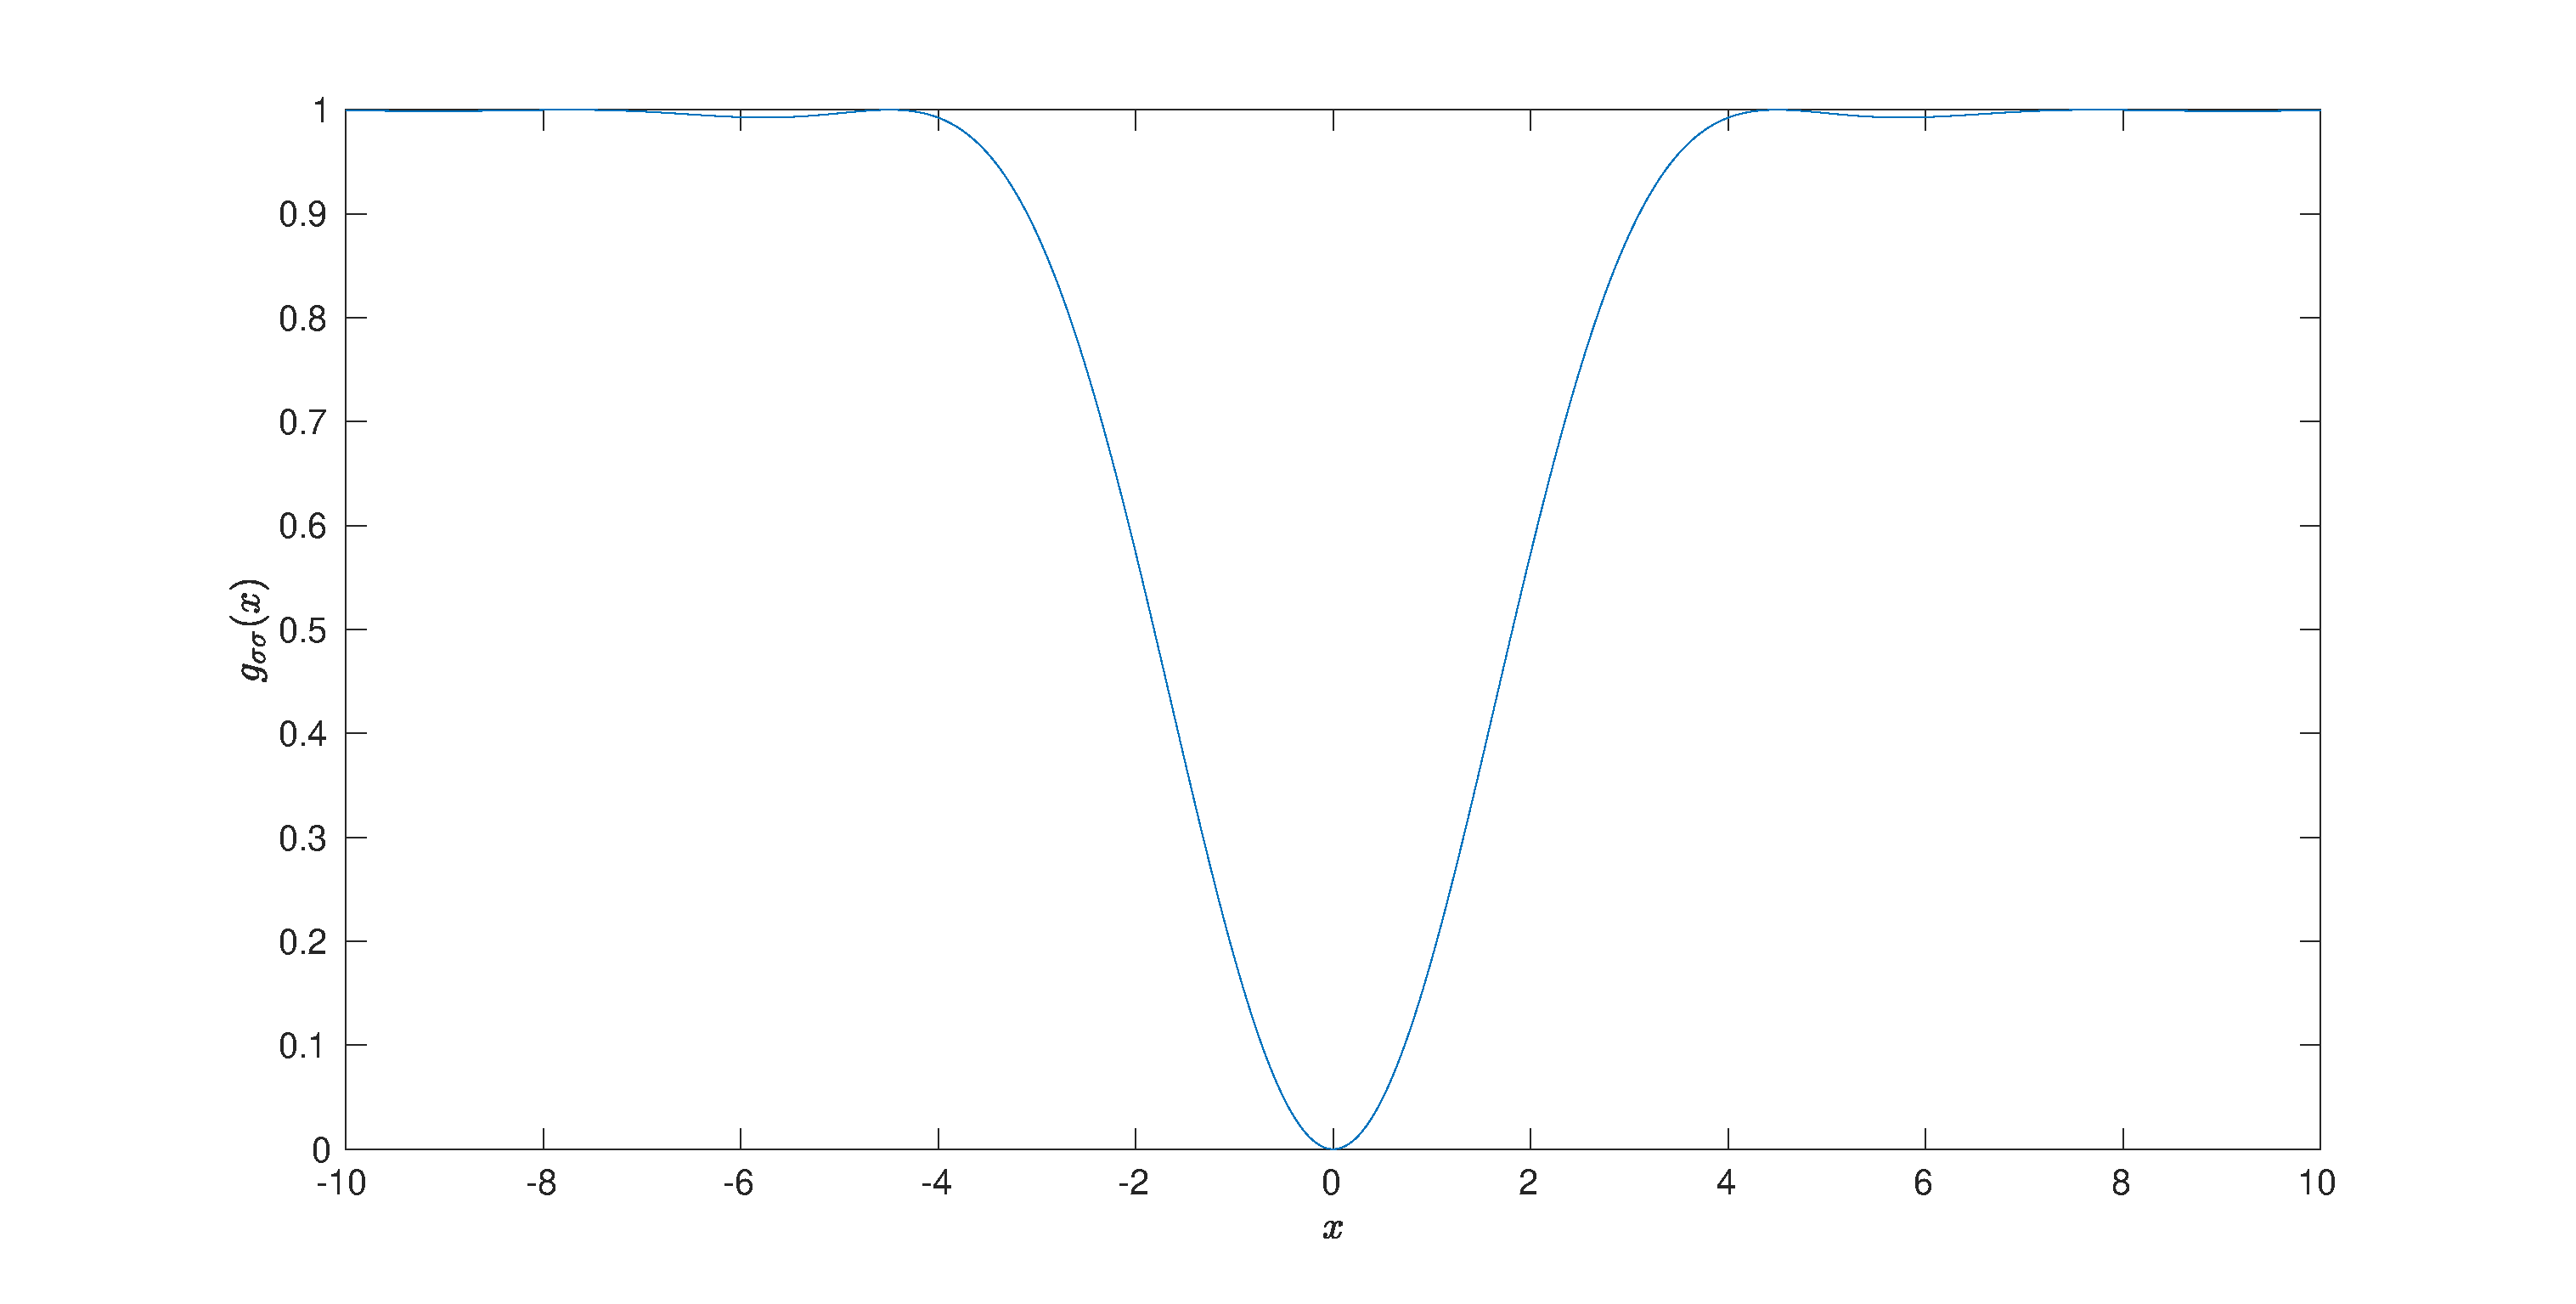
\includegraphics[width=\textwidth]{Density}
\end{figure}
\end{frame}

\begin{frame}{Example frame 1}
This is the first frame
\end{frame}

\begin{frame}{Example frame 2}
\begin{block}{Example block}
\begin{itemize}
\item item 1
\item item 2
\end{itemize}
\end{block}
\end{frame}

\end{document}
